\section{Recursion}

Suppose we have the following knowledge base:

\begin{codeblock}
parent(terach, abraham).
parent(abraham, isaac).
parent(isaac, jacob).
parent(jacob, joseph).
...
\end{codeblock}

We want to define a predicate \hltext{ancestor/2} as \texttt{ancestor(X,Y)} that is true when \texttt{X} is an ancestor of \texttt{Y}.

If we think about it, a parent is considered an ancestor, so maybe we can just write:

\begin{codeblock}
ancestor(X, Y) :- parent(X, Y).
\end{codeblock}

But a grandparent is also an ancestor!

\begin{codeblock}
ancestor(X, Z) :- parent(X, Y), parent(Y, Z).
\end{codeblock}

And a great-grandparent!

\begin{codeblock}
ancestor(X, W) :- parent(X, Y), parent(Y, Z), parent(Z, W).
\end{codeblock}

And $\dots$

\problembox{
With this approach, we can only capture a specific chain of generations (here we only captured 3). What if someone asks about a chain of 10 generations? or 100? or ...? $\leadsto$ infinite number of rules needed!
}

\solutionbox{
Recursion to the rescue $\leadsto$ Think Recursively!
}

We define the ancestor relation recursively. First, we define the \textbf{base case}: $X$ is an ancestor of $Y$ if $X$ is the immediate parent of $Y$:

\begin{codeblock}
ancestor(X, Y) :-
    parent(X, Y).
\end{codeblock}

Now we define the \textbf{recursive case}: $X$ is an ancestor of $Y$ if $X$ is a parent of some intermediate person $Z$, and $Z$ is an ancestor of $Y$!

\begin{codeblock}
ancestor(X, Y) :-
    parent(X, Z),
    ancestor(Z, Y).
\end{codeblock}

\subsection{Recursion in Imperative Programming}

Let us review recursion in Python to remember how call stacks work procedurally. Recursion means a function calls itself to solve smaller parts of a problem until it reaches a \textbf{base case}, which stops the recursion. Every recursive function needs:
\begin{enumerate}
    \item A \textbf{base case} (when to stop).
    \item A \textbf{recursive case} (when to keep calling itself).
\end{enumerate}

\begin{example}[Factorial]{}
Mathematically, factorial is recursive:
\[
n! = n \times (n - 1)! \quad \text{with the base case} \quad 0! = 1
\]

We translate that to a Python program:

\begin{codeblock}
def factorial(n):
    # Base case
    if n == 0:
        return 1
    # Recursive case
    return n * factorial(n - 1)
\end{codeblock}

Let's trace \texttt{factorial(4)}:
\[
\begin{aligned}
\text{factorial}(4) &= 4 \times \text{factorial}(3) \\
             &= 4 \times (3 \times \text{factorial}(2)) \\
             &= 4 \times (3 \times (2 \times \text{factorial}(1))) \\
             &= 4 \times (3 \times (2 \times (1 \times \text{factorial}(0)))) \\
             &= 4 \times (3 \times (2 \times (1 \times 1))) = 24
\end{aligned}
\]
\end{example}

\observationbox{
Each call pauses until the smaller call finishes. The recursion \textit{"unwinds"} once it hits the base case.
}

\begin{example}[Fibonacci]{}
The Fibonacci sequence is defined as:
\[
F(0) = 0, \quad F(1) = 1, \quad F(n) = F(n - 1) + F(n - 2) \text{ for }n\geq 2
\]

In Python:

\begin{codeblock}
def fibonacci(n):
    # Base cases
    if n == 0:
        return 0
    elif n == 1:
        return 1
    # Recursive case
    return fibonacci(n - 1) + fibonacci(n - 2)
\end{codeblock}

Tracing \texttt{fibonacci(4)}:

\[
\begin{aligned}
\text{fibonacci}(4) &= \text{fibonacci}(3) + \text{fibonacci}(2) \\
             &= (\text{fibonacci}(2) + \text{fibonacci}(1)) + (\text{fibonacci}(1) + \text{fibonacci}(0)) \\
             &= ((\text{fibonacci}(1) + \text{fibonacci}(0)) + 1) + (1 + 0) \\
             &= ((1 + 0) + 1) + (1 + 0) = 3
\end{aligned}
\]
\end{example}

\observationbox{
Here you can see multiple recursive branches forming a call tree, because each call spawns two more calls.
}

\titledbox{Tail Recursion}{
In \textbf{tail recursion}, the recursive call is the \textit{last operation} performed in the function. There is no computation left after the recursive call returns.  
This allows certain languages (not Python, but others like Scheme or Prolog) to reuse the same stack frame, converting recursion into an iterative process internally. This is known as \textbf{tail call optimization (TCO)}.
}

\titledbox{Accumulator}{
A clean way to express tail recursion is by defining a \textbf{main function} that delegates to a \textbf{helper} carrying an \textbf{accumulator}. The helper performs the recursion, while the main function provides the initial accumulator value.
}

\begin{example}[Factorial]{}
Here is a tail-recursive implementation of the \texttt{fact} function:
\begin{codeblock}
def fact(n):
    def fact_helper(n, acc):
        # Base case
        if n == 0:
            return acc
        # Tail-recursive case
        return fact_helper(n - 1, n * acc)
    return fact_helper(n, 1)
\end{codeblock}

Tracing \texttt{fact(4)}:

\[
\begin{aligned}
\texttt{fact}(4) &= \texttt{fact\_helper}(4, 1) \\
        &\rightarrow \texttt{fact\_helper}(3, 4) \\
        &\rightarrow \texttt{fact\_helper}(2, 12) \\
        &\rightarrow \texttt{fact\_helper}(1, 24) \\
        &\rightarrow \texttt{fact\_helper}(0, 24) = 24
\end{aligned}
\]
\end{example}

\observationbox{
Each recursive call directly returns another call without additional computation. This makes the recursion tail-recursive, and languages with TCO can execute it in constant stack space.
}

\begin{example}[Fibonacci]{}
We can apply the same structure to the Fibonacci sequence.  
The helper carries the previous two Fibonacci numbers as parameters \texttt{(a, b)} (think of them as two pointers, \texttt{prev} and \texttt{current}).
\begin{codeblock}
def fib(n):
    def fib_helper(n, a, b):
        # Base case
        if n == 0:
            return a
        # Tail-recursive case
        return fib_helper(n - 1, b, a + b)
    return fib_helper(n, 0, 1)
\end{codeblock}
Tracing \texttt{fib(5)}:
\[
\begin{aligned}
fib(5) &= fib\_helper(5, 0, 1) \\
       &\rightarrow fib\_helper(4, 1, 1) \\
       &\rightarrow fib\_helper(3, 1, 2) \\
       &\rightarrow fib\_helper(2, 2, 3) \\
       &\rightarrow fib\_helper(1, 3, 5) \\
       &\rightarrow fib\_helper(0, 5, 8) = 5
\end{aligned}
\]
\end{example}

\observationbox{
Here, \texttt{a} represents the previous Fibonacci number and \texttt{b} the current one. Each call shifts these accumulators forward until the base case is reached. See \figref{fig:fib_tail_recursion} for illustration.
}

\titledbox{Tip}{
Keep this accumulator pattern in mind: in upcoming sections on arithmetic and list processing, we will see how Prolog leverages accumulators to execute recursive predicates in constant stack space via \textbf{Last Call Optimization (LCO)}.
}

\begin{figure}[H]
    \centering
    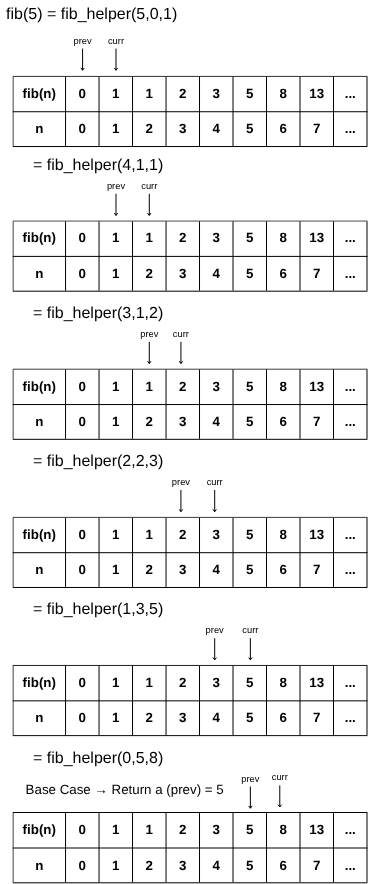
\includegraphics[width=0.3\linewidth]{images/fib_tail_recursion.png}
    \caption{Fib Tail Recursion}
    \label{fig:fib_tail_recursion}
\end{figure}

